%
% $RCSfile: separation_of_concerns.tex,v $
%
% Copyright (C) 2002-2008. Christian Heller.
%
% Permission is granted to copy, distribute and/or modify this document
% under the terms of the GNU Free Documentation License, Version 1.1 or
% any later version published by the Free Software Foundation; with no
% Invariant Sections, with no Front-Cover Texts and with no Back-Cover
% Texts. A copy of the license is included in the section entitled
% "GNU Free Documentation License".
%
% http://www.cybop.net
% - Cybernetics Oriented Programming -
%
% http://www.resmedicinae.org
% - Information in Medicine -
%
% Version: $Revision: 1.1 $ $Date: 2008-08-19 20:41:08 $ $Author: christian $
% Authors: Christian Heller <christian.heller@tuxtax.de>
%

\subsection{Separation of Concerns}
\label{separation_of_concerns_heading}
\index{Separation of Concerns}
\index{SoC}
\index{Container}
\index{Component}
\index{Contract}
\index{Separation of Contract and Implementation}
\index{Concern}
\index{Component Oriented Programming}
\index{COP}
\index{Role of a Component}
\index{Electronic Health Record}
\index{EHR}
\index{Service Manager for Components}
\index{Lookup Method identifying Components}
\index{Fully Qualified Name}
\index{FQN}
\index{Component Selector}

The \emph{Avalon} project \cite{avalon} writes:

\begin{quote}
    Separation of concerns in its simplest form is separating a problem into
    different points of view. Every time one uses interfaces within object- or
    component oriented programming, the \emph{Separation of Concerns} (SoC)
    pattern is applied. The interface separates the implementation concern from
    the concern of the user of the interface.
\end{quote}

Interfaces \emph{pool} common methods (section \ref{classification_heading}).
Inheriting an interface, components indicate to their surrounding container
which methods they implement so that the container can use and rely on these.
Therefore, one often talks of a \emph{Contract} between container and
component. The contract defines what the container (as user of the component)
must provide and what the component produces. In the end, the separation of
\emph{Interface and Implementation} (section
\ref{interface_and_implementation_heading}) could be more correctly called
separation of \emph{Contract and Implementation}.

The contract was mentioned in section \ref{component_lifecycle_heading} which
explained that a container is responsible for taking its components through a
lifecycle. The \emph{Avalon} project \cite{avalon} specifies a number of
concerns which enforce the implementation of one or more lifecycle methods.
Here is a list of some concerns referring to the methods of section
\ref{component_lifecycle_heading}:

\begin{itemize}
    \item[-] Loggable
    \item[-] Contextualizable
    \item[-] Composable
    \item[-] Configurable
    \item[-] Initializable
    \item[-] Startable
    \item[-] Suspendable
\end{itemize}

For example, an object that can be configured implements the \emph{Configurable}
interface. The contract surrounding that interface is that the container as
instantiator of the object passes a \emph{Configuration} object to the component
being a configurable object. Just what the configurable object does with the
passed configuration object is irrelevant to the instantiator.

\begin{figure}[ht]
    \begin{center}
        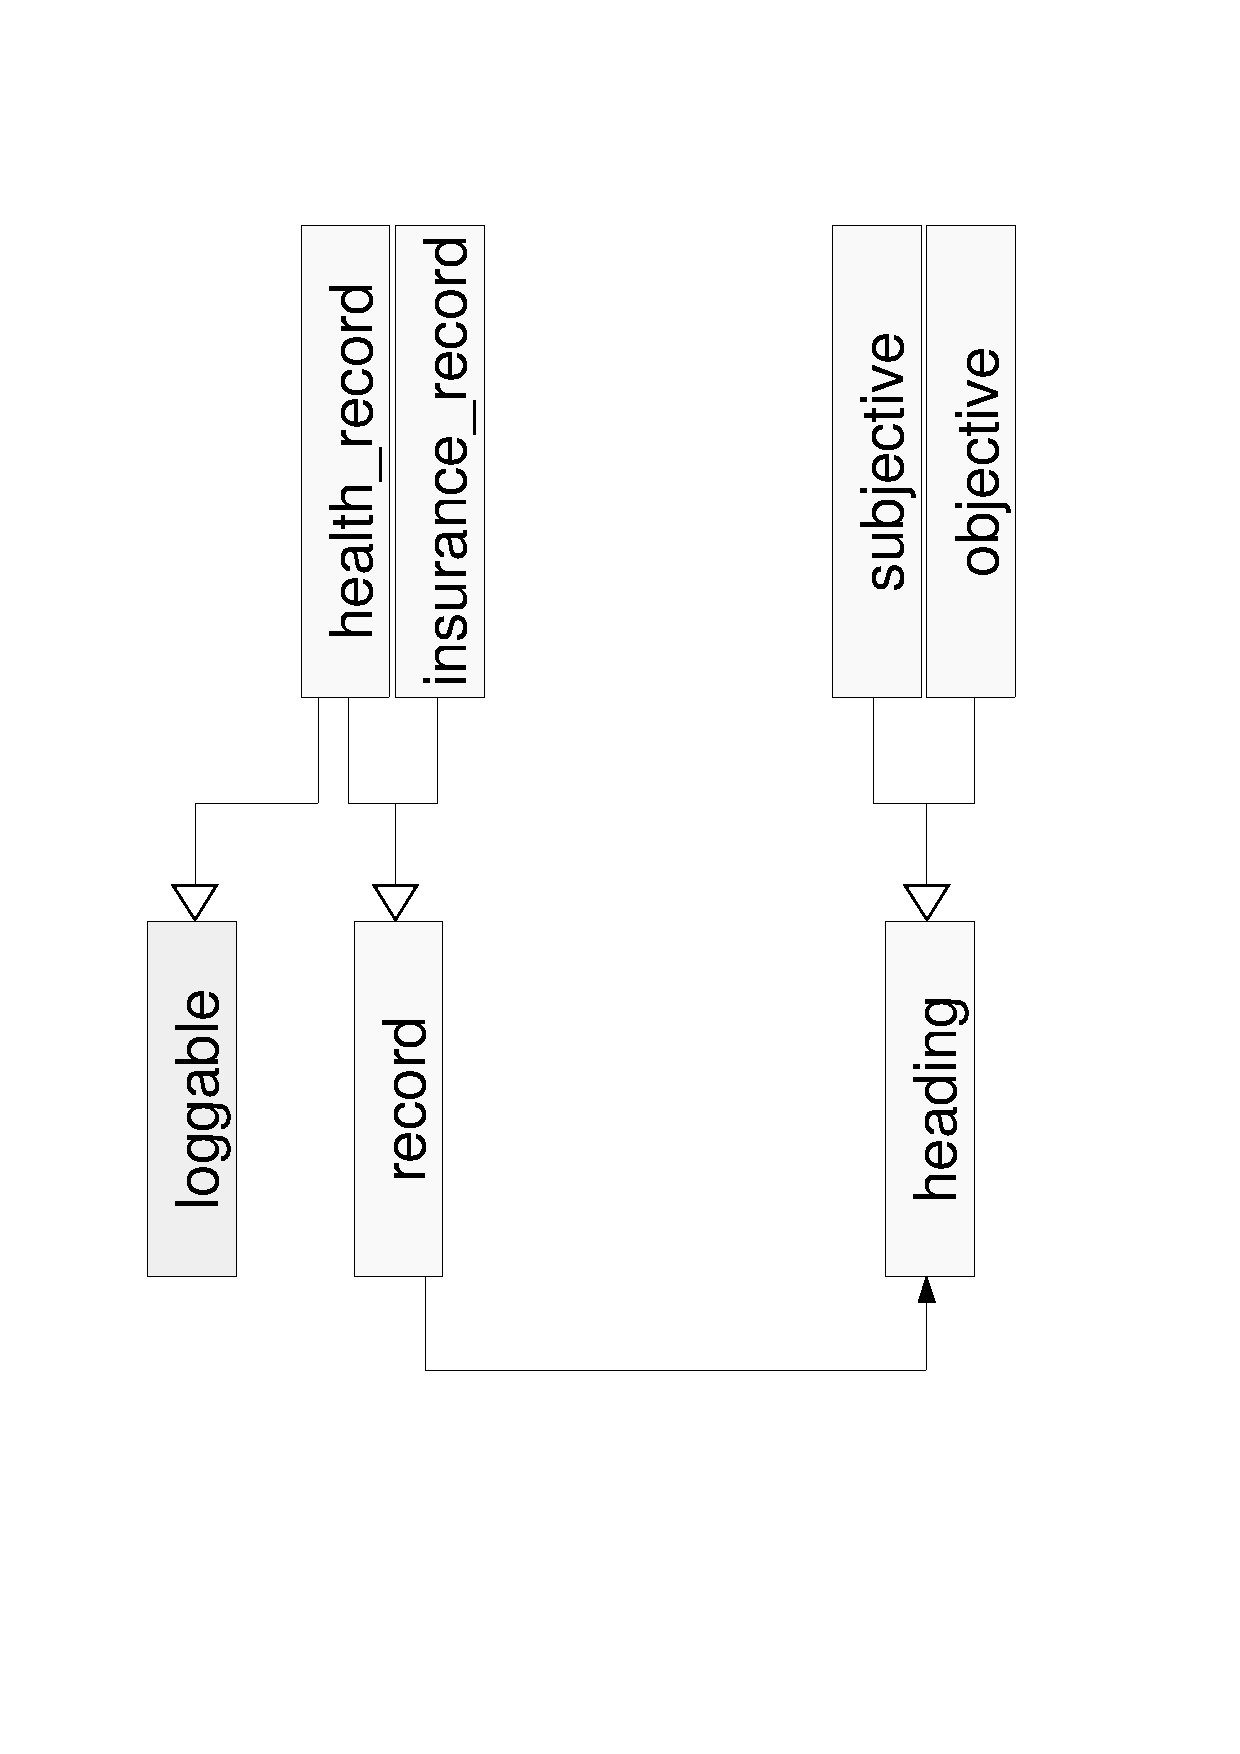
\includegraphics[scale=0.3,angle=-90]{graphic/concern.pdf}
        \caption{Class Inheriting Loggable Concern Interface}
        \label{concern_figure}
    \end{center}
\end{figure}

Figure \ref{concern_figure} shows an \emph{Electronic Health Record} (EHR)
component implementing the \emph{Loggable} interface which indicates that the
component offers functionality for the logging of messages. To fully explain
the figure: The EHR inherits from a general \emph{Record} class that references
so-called \emph{Heading} objects which may be a \emph{Subjective} description
of a patient or an \emph{Objective} result of an examination. Of course, these
objects may be programmed as components as well.

A common comparison used in component oriented programming is that of the
\emph{Role} coming from theater \cite{avalon}. The function or action of a
component's role within a system, as well as its contracts, are defined by its
script -- the interface. Any object that implements the component interface
must comply with the contracts. This allows developers to manipulate components
using a standard interface, without worrying about the semantics of the
implementation. They are separate concerns.

A \emph{Service Manager} is often used to get an instance of the needed
component. The manager's \emph{lookup} method identifies the component based on
the \emph{Fully Qualified Name} (FQN) of the role (interface). If several
components functioning in the same role exist, a \emph{Component Selector} may
be applied to choose the right one. More details are given in \cite{avalon}.
